\documentclass[12pt]{article}
\usepackage[table]{xcolor}
\usepackage[shortlabels]{enumitem}
\usepackage{tabularx,xltabular}
\usepackage{graphicx}
\usepackage{hyperref}
\usepackage{verbatim}
\usepackage{geometry}
\usepackage{ulem}
\usepackage[official]{eurosym}
\usepackage{tikz}
\usetikzlibrary{arrows,backgrounds,calc,decorations.markings,patterns,3d,positioning,fit,angles, quotes}
\usepackage{pgfplots}
\pgfplotsset{compat = newest}
\usetikzlibrary{fit}
\newcommand\addvmargin[1]{
\usetikzlibrary{arrows}
\node[fit=(current bounding box),inner ysep=#1,inner xsep=0]{};}
\usepackage{cancel}
\usepackage{fontspec}
\usepackage{array}  
\geometry{a4paper, top=2cm, left=2cm, right=2cm, bottom=2cm, headsep=1cm}
\usepackage{tabu}
\usepackage{pst-node}
\usepackage{colortbl}
\usepackage{array}
\usepackage{german}
\setlength\parindent{0pt}
\newcolumntype{?}{!{\vrule width 1pt}}
\usepackage{makecell}
\renewcommand{\arraystretch}{2.5}
\usepackage{pbox}
\usepackage{amssymb}
\usepackage{amsmath}
\usepackage{booktabs}
\newcolumntype{L}[1]{>{\raggedright\let\newline\\\arraybackslash\hspace{0pt}}m{#1}}
\newcolumntype{C}[1]{>{\centering\let\newline\\\arraybackslash\hspace{0pt}}m{#1}}
\newcolumntype{R}[1]{>{\raggedleft\let\newline\\\arraybackslash\hspace{0pt}}m{#1}}
\begin{document}
\rightline{Datum: 08.12.2023}
\centerline{{\Large Üben für die Arbeit}} 
\vspace{1cm}
\noindent \\


\begin{xltabular}{\textwidth}{|C{0.75cm}|X|C{0.75cm}|X|}
\arrayrulecolor{black}\hline
a)&Setze für die Variabel b den Wert -7 ein und berechne den Wert des Terms:$$5 \cdot b - 5 \cdot b$$
&
b)&Setze für die Variabel x den Wert 9 ein und berechne den Wert des Terms:$$5 \cdot x - 2$$
\\\hline
c)&Vereinfache:$$3a + 2a - 4a=?$$
&
d)&Vereinfache:$$3a + 3 + 1 + 1=?$$
\\\hline
e)&Berechne die Variable $$10\cdot a-20=10$$
&
f)&Berechne die Variable $$2\cdot b-19=-9$$
\\\hline
g)&\pbox{6cm}{Bestimme den Umfang und die Fläche von: \\\tikzstyle{background grid}=[draw, black!15,step=.5cm]
\noindent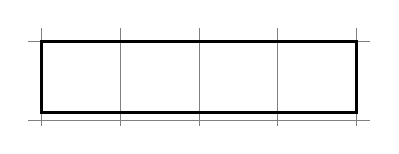
\begin{tikzpicture}[show background grid]
\draw[black, very thick] (0cm,0.1cm) rectangle (4cm,1cm);
\end{tikzpicture}}
&
h)&\pbox{5cm}{
Berechne den Flächeninhalt von:\\
\tikzstyle{background grid}=[draw, black!15,step=.5cm]
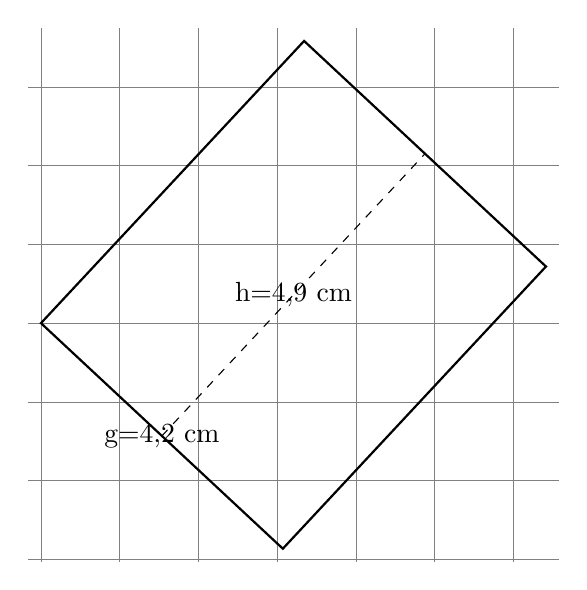
\begin{tikzpicture}[show background grid]
\draw[thick,black,rotate=317] (0,0) -- node{g=4,2 cm} ++(4.2,0) -- ++(0.0,4.9) -- ++(-4.2,0) --cycle;
\draw[dashed,black,rotate=317] (2.1,0)  -- node{h=4,9 cm} ++(0,4.9);
\end{tikzpicture}
}
\\\hline
i)&\pbox{5cm}{
Berechne den Flächeninhalt von:\\
\tikzstyle{background grid}=[draw, black!15,step=.5cm]
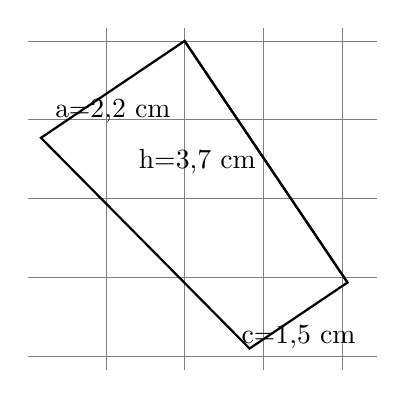
\begin{tikzpicture}[show background grid]
\draw[thick,black,rotate=214] (0,0) -- node[below]{a=2,2 cm} ++(2.2,0) -- ++(-0.7,3.7) --node[below]{c=1,5 cm} ++(-1.5,0) --cycle;
\draw[thick,black,rotate=214] (2.220446049250313e-16,0) --node[left]{h=3,7 cm}  ++(0,3.7);
\end{tikzpicture}
}
&
j)&\pbox{5cm}{
Berechne den Flächeninhalt von:\\
\tikzstyle{background grid}=[draw, black!15,step=.5cm]
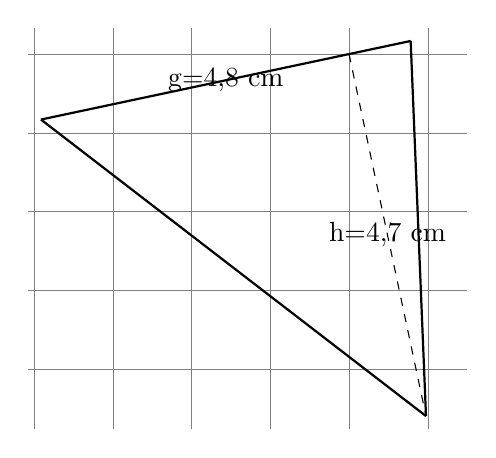
\begin{tikzpicture}[show background grid]
\draw[thick,black] (192:-0.7999999999999998) -- node{g=4,8 cm} (192:4.0);
\draw[thick,black] (192:-0.7999999999999998)  -- (282:4.7);
\draw[thick,black] (192:4.0)  -- (282:4.7);
\draw[dashed,black] (0,0)  -- node{h=4,7 cm} (282:4.7);
\draw[dashed,black] (0,0)  -- (192:-0.7999999999999998);
\end{tikzpicture}
}
\\\hline
k)&\pbox{5cm}{
Berechne den Flächeninhalt von:\\
\tikzstyle{background grid}=[draw, black!15,step=.5cm]
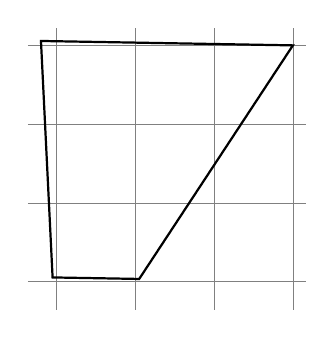
\begin{tikzpicture}[show background grid]
\draw[thick,black,rotate=179] (0,0) -- node[below]{} ++(3.2,0) -- ++(-0.2,3.0) --node[below]{} ++(-1.1,0) --cycle;
\end{tikzpicture}
}
&
l)&\pbox{5cm}{
Berechne den Flächeninhalt von:\\
\tikzstyle{background grid}=[draw, black!15,step=.5cm]
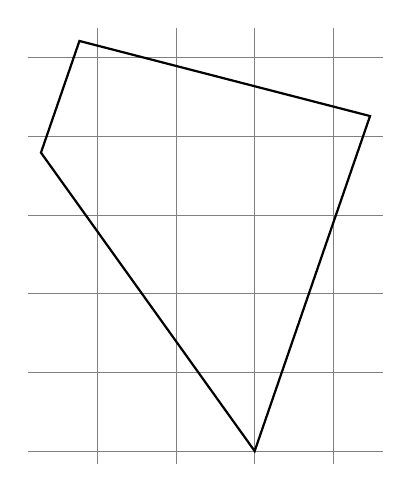
\begin{tikzpicture}[show background grid]
\draw[thick,black,rotate=71] (0,0) -- node[below]{} ++(4.5,0) -- ++(-0.3,3.8) --node[below]{} ++(-1.5,0) --cycle;
\end{tikzpicture}
}
\\\hline
m)&Stelle die Flächenformel des Dreiecks nach der fehlenden Seite um und berechne diese und den Umfang für $A=7,705~cm^2$, $a=1,5~cm$, $b=9,6~cm$  und $h_c=2,3~cm$.
&
n)&Stelle die Umfangsformel des Rechtecks nach der fehlenden Seite um und berechne diese und den Flächeninhalt für $u=23~cm$ und $a=2,6~cm$.
\\\hline
\end{xltabular}
\vspace{0.5cm}
\newpage
\rightline{Datum: 08.12.2023}
\centerline{{\large Lösungen Üben für die Arbeit}} 
\vspace{0.5cm}

\begin{xltabular}{\textwidth}{|C{0.75cm}|X|C{0.75cm}|X|}
\arrayrulecolor{black}\hline
a)&$\begin{aligned}
\textcolor{red}{b=-7} & \rightarrow\\
5 \cdot b - 5 \cdot b=&5 \cdot \textcolor{red}{(-7)} - 5 \cdot \textcolor{red}{(-7)}=0\\
\end{aligned}$
&
b)&$\begin{aligned}
\textcolor{red}{x=9} & \rightarrow\\
5 \cdot x - 2=&5 \cdot \textcolor{red}{9} - 2=43\\
\end{aligned}$
\\\hline
c)&$3a + 2a - 4a=a$
&
d)&$3a + 3 + 1 + 1=3a + 5$
\\\hline
e)&\begingroup\setlength{\jot}{-0.03cm}
\tikzstyle{background grid}=[draw, black!15,step=.5cm]
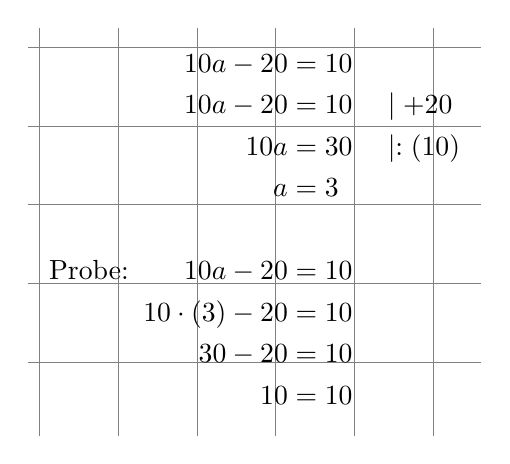
\begin{tikzpicture}[show background grid]
\node[below right] at (0,0.1) {
$\begin{aligned}
10a-20 &=10& &  \\
10a - 20 &=10& & \mid + 20\\
10a &=30& & \mid :\left(10\right)\\
a &=3& & 
\\
\\
\mbox{Probe:}\qquad 10a-20 &=10& &  \\
10\cdot \left(3\right)-20 &=10& &  \\
30-20 &=10& &  \\
10 &=10& &  \\
\end{aligned}$};
\end{tikzpicture}
\endgroup
&
f)&\begingroup\setlength{\jot}{-0.03cm}
\tikzstyle{background grid}=[draw, black!15,step=.5cm]
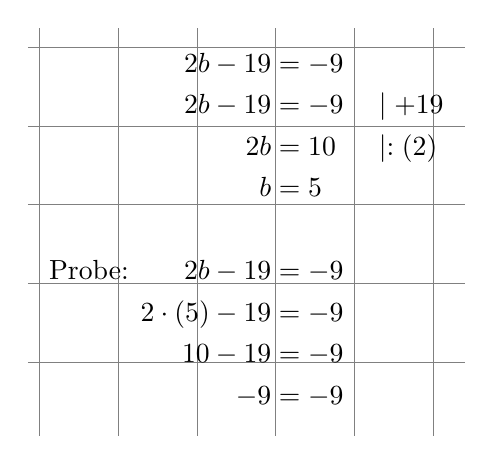
\begin{tikzpicture}[show background grid]
\node[below right] at (0,0.1) {
$\begin{aligned}
2b-19 &=-9& &  \\
2b - 19 &=-9& & \mid + 19\\
2b &=10& & \mid :\left(2\right)\\
b &=5& & 
\\
\\
\mbox{Probe:}\qquad 2b-19 &=-9& &  \\
2\cdot \left(5\right)-19 &=-9& &  \\
10-19 &=-9& &  \\
-9 &=-9& &  \\
\end{aligned}$};
\end{tikzpicture}
\endgroup
\\\hline
g)&\pbox{6cm}{$U=2\cdot a+2\cdot b$ \\ $U=2\cdot4cm+2\cdot1cm=10cm$ \\$A=a\cdot b$ \\ $A=4\cdot1=4cm^2$ \\\tikzstyle{background grid}=[draw, black!15,step=.5cm]
\noindent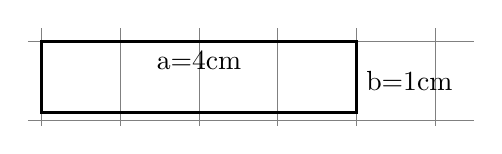
\begin{tikzpicture}[show background grid]
\draw[black, very thick] (0cm,0.1cm) rectangle (4cm,1cm);
\draw (2.0cm,1cm) node[below]{a=4cm}; 
\draw (4cm,0.5cm) node[right]{b=1cm}; 
\end{tikzpicture}}
&
h)&\pbox{5cm}{
$\begin{aligned}
geg.: g&=4,2 cm \\
   h&=4,9 cm \\
ges.: A&=? \\
A&=g\cdot h \\
&=4,2\cdot 4,9 \\
\makebox[0pt][l]{\uuline{\phantom{$A=20,58~cm^2$} } }
A&=20,58~cm^2
\end{aligned}$
\tikzstyle{background grid}=[draw, black!15,step=.5cm]
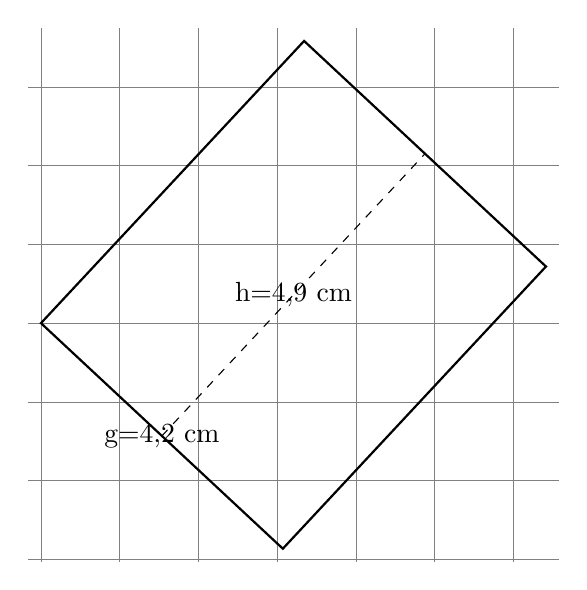
\begin{tikzpicture}[show background grid]
\draw[thick,black,rotate=317] (0,0) -- node{g=4,2 cm} ++(4.2,0) -- ++(0.0,4.9) -- ++(-4.2,0) --cycle;
\draw[dashed,black,rotate=317] (2.1,0)  -- node{h=4,9 cm} ++(0,4.9);
\end{tikzpicture}
}
\\\hline
i)&\pbox{5cm}{
\tikzstyle{background grid}=[draw, black!15,step=.5cm]
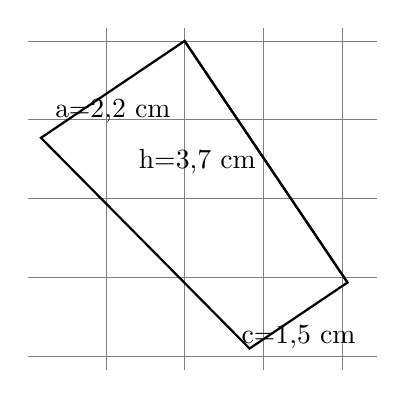
\begin{tikzpicture}[show background grid]
\draw[thick,black,rotate=214] (0,0) -- node[below]{a=2,2 cm} ++(2.2,0) -- ++(-0.7,3.7) --node[below]{c=1,5 cm} ++(-1.5,0) --cycle;
\draw[thick,black,rotate=214] (2.220446049250313e-16,0) --node[left]{h=3,7 cm}  ++(0,3.7);
\end{tikzpicture}
$\begin{aligned}
geg.: a&=2,2 cm \\
   c&=1,5 cm \\
   h&=3,7 cm \\
ges.: A&=? \\
A&=\frac{a+c}{2}\cdot h \\
&=\frac{2,2+1,5}{2}\cdot3,7\\
\makebox[0pt][l]{\uuline{\phantom{$A=6,85~cm^2$} } }
A&=6,85~cm^2
\end{aligned}$
}
&
j)&\pbox{5cm}{
$\begin{aligned}
geg.: g&=4,8 cm \\
   h&=4,7 cm \\
ges.: A&=? \\
A&=\frac{g \cdot h}{2} \\
&=4,8 \cdot \frac{4,7}{2}\\
\makebox[0pt][l]{\uuline{\phantom{$A=11,28~cm^2$} } }
A&=11,28~cm^2
\end{aligned}$
\tikzstyle{background grid}=[draw, black!15,step=.5cm]
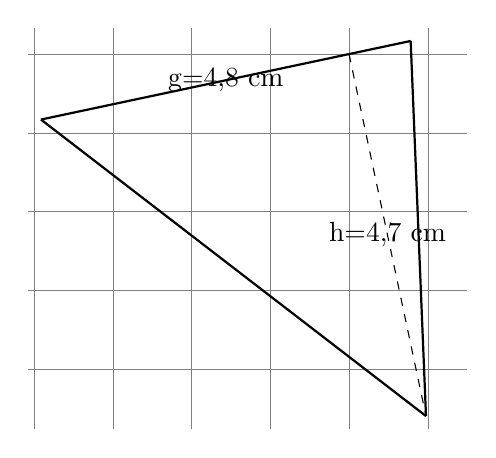
\begin{tikzpicture}[show background grid]
\draw[thick,black] (192:-0.7999999999999998) -- node{g=4,8 cm} (192:4.0);
\draw[thick,black] (192:-0.7999999999999998)  -- (282:4.7);
\draw[thick,black] (192:4.0)  -- (282:4.7);
\draw[dashed,black] (0,0)  -- node{h=4,7 cm} (282:4.7);
\draw[dashed,black] (0,0)  -- (192:-0.7999999999999998);
\end{tikzpicture}
}
\\\hline
k)&\pbox{5cm}{
\tikzstyle{background grid}=[draw, black!15,step=.5cm]
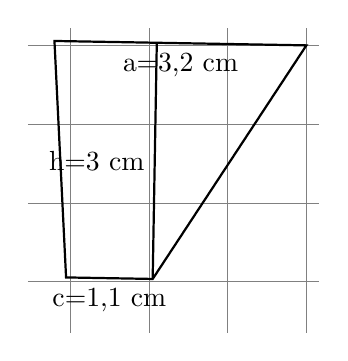
\begin{tikzpicture}[show background grid]
\draw[thick,black,rotate=179] (0,0) -- node[below]{a=3,2 cm} ++(3.2,0) -- ++(-0.2,3.0) --node[below]{c=1,1 cm} ++(-1.1,0) --cycle;
\draw[thick,black,rotate=179] (1.9000000000000001,0) --node[left]{h=3 cm}  ++(0,3.0);
\end{tikzpicture}
$\begin{aligned}
geg.: a&=3,2 cm \\
   c&=1,1 cm \\
   h&=3 cm \\
ges.: A&=? \\
A&=\frac{a+c}{2}\cdot h \\
&=\frac{3,2+1,1}{2}\cdot3\\
\makebox[0pt][l]{\uuline{\phantom{$A=6,45~cm^2$} } }
A&=6,45~cm^2
\end{aligned}$
}
&
l)&\pbox{5cm}{
\tikzstyle{background grid}=[draw, black!15,step=.5cm]
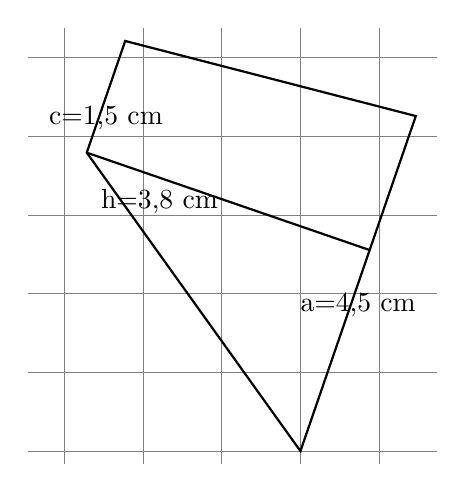
\begin{tikzpicture}[show background grid]
\draw[thick,black,rotate=71] (0,0) -- node[below]{a=4,5 cm} ++(4.5,0) -- ++(-0.3,3.8) --node[below]{c=1,5 cm} ++(-1.5,0) --cycle;
\draw[thick,black,rotate=71] (2.7,0) --node[left]{h=3,8 cm}  ++(0,3.8);
\end{tikzpicture}
$\begin{aligned}
geg.: a&=4,5 cm \\
   c&=1,5 cm \\
   h&=3,8 cm \\
ges.: A&=? \\
A&=\frac{a+c}{2}\cdot h \\
&=\frac{4,5+1,5}{2}\cdot3,8\\
\makebox[0pt][l]{\uuline{\phantom{$A=11,4~cm^2$} } }
A&=11,4~cm^2
\end{aligned}$
}
\\\hline
m)&\tikzstyle{background grid}=[draw, black!15,step=.5cm]
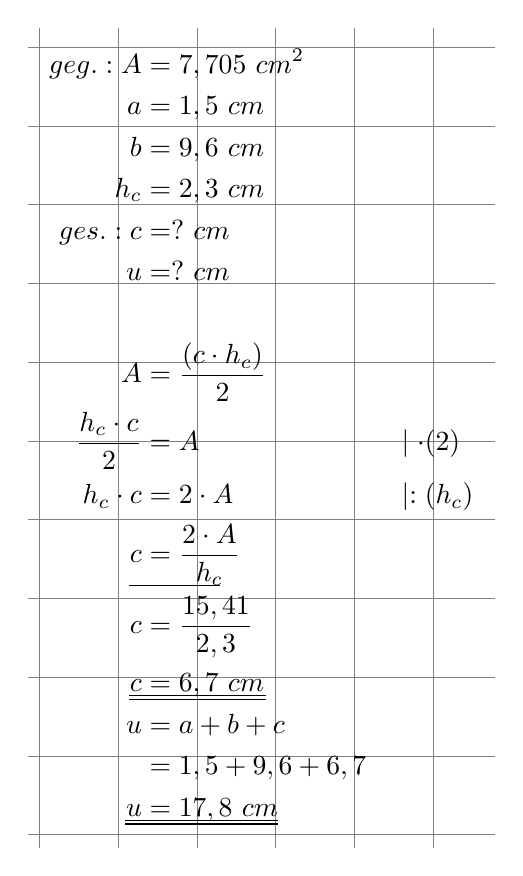
\begin{tikzpicture}[show background grid]
\node[below right] at (0,0.1) {
$\begin{aligned}
geg.: A &=7,705~cm^2& & \\
  a &=1,5~cm& & \\
  b &=9,6~cm& & \\
  h_c &=2,3~cm& & \\
ges.: c &=?~cm& & \\
u &=?~cm& & \\
& & & \\
A &={{\frac{\left(c\cdot h_c\right)}{2}}}& & \\
{{\frac{h_c\cdot c}{2}}} &=A& & \mid \cdot (2)\\
h_c\cdot c &=2\cdot A& & \mid :(h_c)\\
\makebox(0pt,-0.25cm)[l]{\uline{\phantom{$c ={{\frac{2\cdot A}{h_c}}}  \\$}}}
c &={{\frac{2\cdot A}{h_c}}}& & \\
c&=\frac{15,41}{2,3}& & \\
\makebox[0pt][l]{\uuline{\phantom{$c=6,7~cm  \\$}}}
c&=6,7~cm& & \\
u&=a+b+c& & \\
&=1,5+9,6+6,7& & \\
\makebox[0pt][l]{\uuline{\phantom{$u=17,8~cm     \\$}}}
u&=17,8~cm   & & \\
\end{aligned}$};
\end{tikzpicture}
&
n)&\tikzstyle{background grid}=[draw, black!15,step=.5cm]
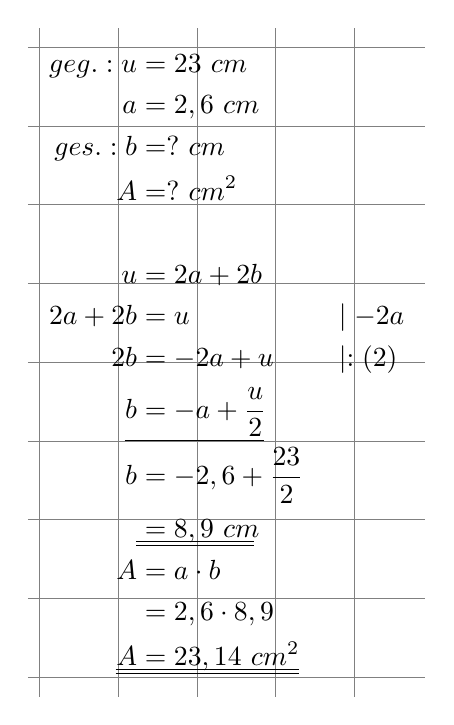
\begin{tikzpicture}[show background grid]
\node[below right] at (0,0.1) {
$\begin{aligned}
geg.: u &=23~cm& & \\
  a &=2,6~cm& & \\
ges.: b &=?~cm& & \\
A &=?~cm^2& & \\
& & & \\
u &=2a+2b& & \\
2a + 2b &=u& & \mid -2a \\
2b &=-2a + u& & \mid :(2)\\
\makebox(0pt,-0.25cm)[l]{\uline{\phantom{$b =-a +{{\frac{ u}{2}}}  \\$}}}
b &=-a +{{\frac{ u}{2}}}& & \\
b&=-2,6+\frac{23}{2}& & \\
\makebox[0pt][l]{\uuline{\phantom{$=8,9~cm  \\$}}}
&=8,9~cm& & \\
A&=a\cdot b & & \\
&=2,6\cdot8,9& & \\
\makebox[0pt][l]{\uuline{\phantom{$A=23,14~cm^2     \\$}}}
A&=23,14~cm^2   & & \\
\end{aligned}$};
\end{tikzpicture}
\\\hline
\end{xltabular}
\vspace{0.5cm}
\end{document}